\documentclass[border=0pt]{standalone}
\usepackage{fontspec}
\setmainfont{Carlito}
\usepackage{unicode-math}
\setmathfont{Latin Modern Math}
\usepackage{xcolor}
\usepackage{booktabs}
\usepackage{tikz}
\usepackage{graphicx}

\definecolor{canvabg}{RGB}{246,244,241}
\definecolor{textDark}{RGB}{40,40,40}
\definecolor{textMute}{RGB}{125,120,113}
\definecolor{accent}{RGB}{18,125,108}
\definecolor{trough}{RGB}{160,55,50}
\definecolor{bridge}{RGB}{30,90,140}

\pagecolor{canvabg}

\providecommand{\Cref}[1]{}
\providecommand{\cref}[1]{}
\providecommand{\ab}[1]{#1}

\renewcommand{\arraystretch}{1.45}

\begin{document}
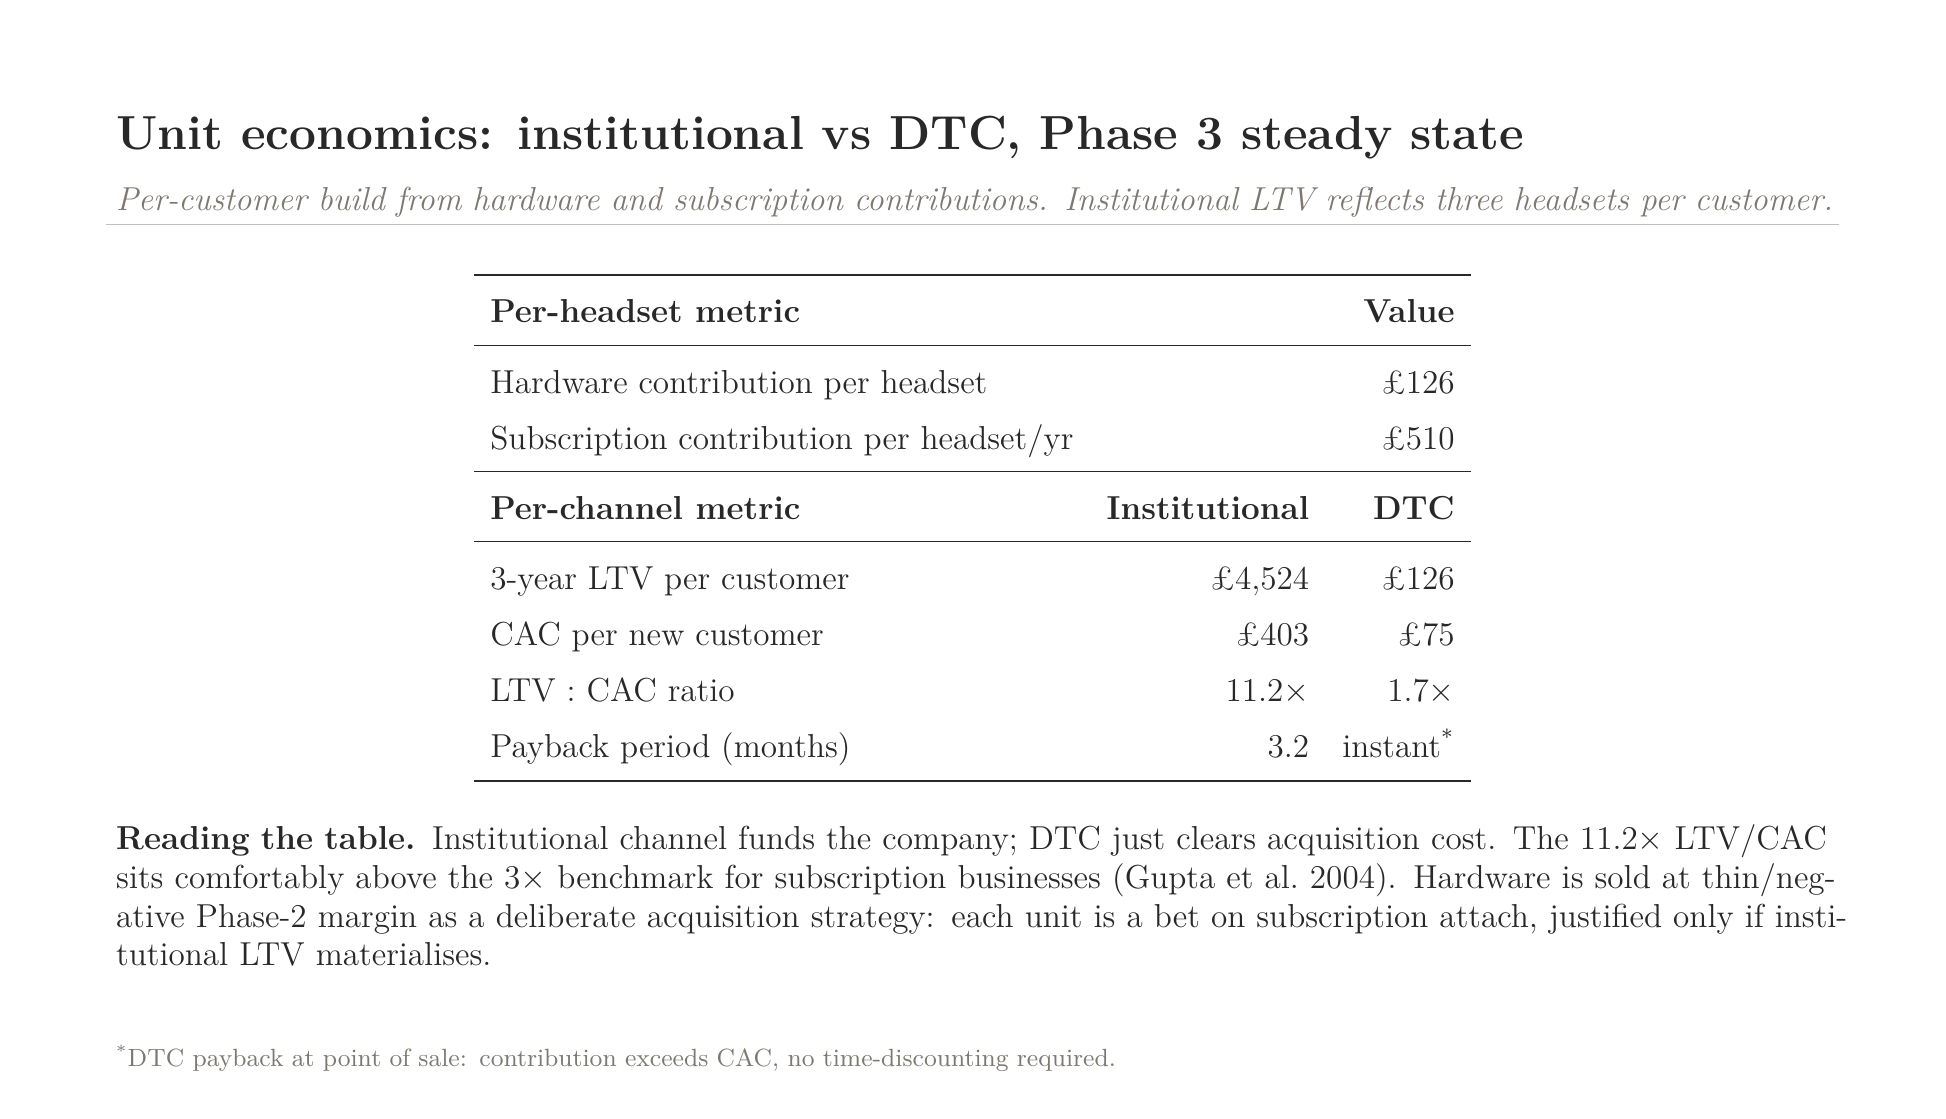
\begin{tikzpicture}[every node/.style={text=textDark}]
\useasboundingbox (0,0) rectangle (24, 13.5);

\node[anchor=north west, font=\bfseries\LARGE] at (1.0, 12.5)
    {Unit economics: institutional vs DTC, Phase 3 steady state};
\node[anchor=north west, font=\itshape\large, text=textMute, text width=22cm]
    at (1.0, 11.6)
    {Per-customer build from hardware and subscription contributions.
     Institutional LTV reflects three headsets per customer.};

\draw[gray!50, line width=0.5pt] (1.0, 11.0) -- (23.0, 11.0);

% Table
\node[anchor=north, font=\large] at (12.0, 10.5) {%
\begin{tabular}{lrr}
    \toprule
    \textbf{Per-headset metric} & \multicolumn{2}{r}{\textbf{Value}} \\
    \midrule
    Hardware contribution per headset        & \multicolumn{2}{r}{\pounds 126} \\
    Subscription contribution per headset/yr & \multicolumn{2}{r}{\pounds 510} \\
    \midrule
    \textbf{Per-channel metric} & \textbf{Institutional} & \textbf{DTC} \\
    \midrule
    3-year LTV per customer                  & \pounds 4{,}524 & \pounds 126 \\
    CAC per new customer                     & \pounds 403       & \pounds 75  \\
    LTV : CAC ratio                          & 11.2$\times$      & 1.7$\times$ \\
    Payback period (months)                  & 3.2               & instant\textsuperscript{*} \\
    \bottomrule
\end{tabular}
};

\node[anchor=north west, text width=22cm, font=\large] at (1.0, 3.5)
    {\textbf{Reading the table.} Institutional channel funds the company;
     DTC just clears acquisition cost. The 11.2$\times$ LTV/CAC sits
     comfortably above the 3$\times$ benchmark for subscription businesses
     (Gupta et al.\ 2004). Hardware is sold at thin/negative Phase-2 margin
     as a deliberate acquisition strategy: each unit is a bet on subscription
     attach, justified only if institutional LTV materialises.};

\node[anchor=north west, font=\small, text=textMute, text width=22cm] at (1.0, 0.7)
    {\textsuperscript{*}DTC payback at point of sale: contribution
     exceeds CAC, no time-discounting required.};

\end{tikzpicture}
\end{document}
